\documentclass[main.tex]{subfiles}
\pagenumbering{arabic}
\newcommand\chapterlabel{ChMIX-statesofmatter}\setcounter{figurenewcounter}{0}\setcounter{tablenewcounter}{0}\setcounter{formulanewcounter}{0}
\setcounter{chapter}{3}

\begin{document}



\chapter[States of matter  ]{States of matter }

\begin{marginfigure}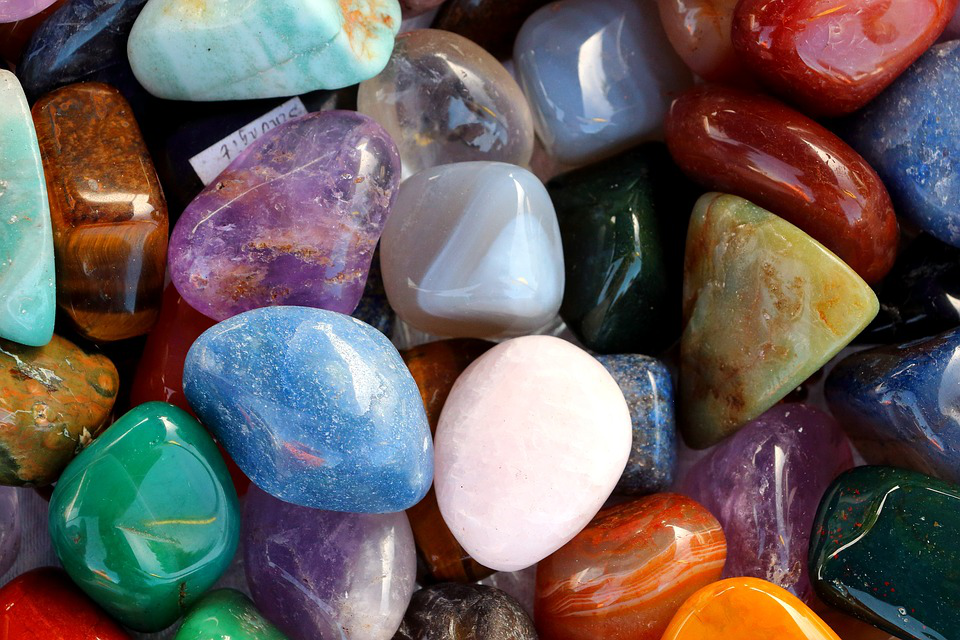
\includegraphics{../Ch-solids/figure1} \end{marginfigure}\import{../Ch-solids/files/}{ChapterIntro}

 \begin{marginfigure}%LEARNING GOALS BOX
 \begin{mytcbox}{GOALS}
%%
%\begin{center}\textcolor{blue}{\faEnvira Chemistry and molecules }\end{center}
%\begin{enumerate}[label=\protect\circled{\color{white}\arabic*}]
%  \import{../Ch-biochemistry/files/}{SectionGoal-Simple-Carbohydrates}
% \import{../Ch-biochemistry/files/}{SectionGoal-Disaccharides-and-polysaccharides}
%\end{enumerate}
%
\renewcommand\chapterlabel{Ch-acidbase}
\begin{center}\textcolor{blue}{\faFlask Acids and bases }\end{center}
\begin{enumerate}[label=\protect\circled{\color{white}\arabic*}]
\import{../\chapterlabel/files/}{SectionGoal-The-PH-scale}
\end{enumerate}


\renewcommand\chapterlabel{Ch-electrolytes}
\begin{center}\textcolor{blue}{\faTint  Electrolytes and solutions }\end{center}
\begin{enumerate}[label=\protect\circled{\color{white}\arabic*}]
\import{../\chapterlabel/files/}{SectionGoal-Solutions-and-composition}
\end{enumerate}
 
\renewcommand\chapterlabel{Ch-thermochemistry}
\begin{center}\textcolor{blue}{\faFire Reactions and energy} \end{center}
\begin{enumerate}[label=\protect\circled{\color{white}\arabic*}]
 \import{../\chapterlabel/files/}{SectionGoal-Energy-temperature}
\end{enumerate}

 
\renewcommand\chapterlabel{Ch-nuclear}
\begin{center}\textcolor{blue}{\faFlash The chemistry of cancer} \end{center}
\begin{enumerate}[label=\protect\circled{\color{white}\arabic*}]
\import{../\chapterlabel/files/}{SectionGoal-Radiation-measurement-units-and-radiation-effects}
	\end{enumerate}

 
	
%\begin{center}\textcolor{blue}{\faGears Let's calculate} \end{center}
%\begin{enumerate}[label=\protect\circled{\color{white}\arabic*}]
%\import{../Ch-measurements/files/}{SectionGoal-Using-Conversion-Factors}
%\end{enumerate}



 \end{mytcbox}
%\vspace{1cm}
%%\begin{tcolorbox}[enhanced,colback=red!5!white,colframe=black!50!red,boxrule=1pt,
%%  arc=0pt,outer arc=0pt,drop heavy lifted shadow]
%%\faGears\ 
%% \import{../Ch-solids/files/}{ChapterDiscussion}
%% \end{tcolorbox}
 \end{marginfigure}%LEARNING GOALS BOX

 \section{\faTint Ions \& ionic charges}
\sloppy\begin{description}
\item[\docfilehook{Mass percent concentration}{}]\import{../Ch-electrolytes/files/}{SubSection-Solutions-and-composition-Mass-percent}
\import{../Ch-electrolytes/problems/}{SampleProblem4}
\item[\docfilehook{Volume percent concentration}{}] \import{../Ch-electrolytes/files/}{SubSection-Solutions-and-composition-Volume-percent-concentration}
\item[\docfilehook{Mass/volume  percent concentration}{}]\import{../Ch-electrolytes/files/}{SubSection-Solutions-and-composition-Massvolume-percent-concentration}
\item[\docfilehook{Molarity concentration}{}]\import{../Ch-electrolytes/files/}{SubSection-Solutions-and-composition-Molarity-concentration}
\import{../Ch-electrolytes/problems/}{SampleProblem5}
\item[\docfilehook{Concentration units as conversion factors}{}]\import{../Ch-electrolytes/files/}{SubSection-Solutions-and-composition-Concentration-units-as-conversion-factors}
\import{../Ch-electrolytes/problems/}{SampleProblem6}
\item[\docfilehook{Dilution}{}]\import{../Ch-electrolytes/files/}{SubSection-Solutions-and-composition-Dilution}
\import{../Ch-electrolytes/problems/}{SampleProblem7}
 \end{description}



\section{The mole}
\import{../Ch-mole/files/}{SectionIntro-The-mole}
\sloppy \begin{description}
\item[\docfilehook{From moles to molecules}{}] \import{../Ch-mole/files/}{SubSection-The-mole-From-moles-to-atoms}
\item[\docfilehook{From molecules to atoms}{}] \import{../Ch-mole/files/}{SubSection-The-mole-From-molecules-to-atoms}
\import{../Ch-mole/problems/}{SampleProblem1} 
\end{description}
	





\section{\faEnvira Converting moles into grams and into atoms}
\import{../Ch-mole/files/}{SectionIntro-Converting-moles-into-grams-and-into-atoms}
\sloppy \begin{description}
\item[\docfilehook{Molar mass of a chemical}{}] \import{../Ch-mole/files/}{SubSection-Converting-moles-into-grams-and-into-atoms-Molar-mass-of-a-chemical}
\import{../Ch-mole/problems/}{SampleProblem2}
\import{../Ch-mole/files/}{SubSection-Converting-moles-into-grams-and-into-atoms-From-moles-to-grams}
\import{../Ch-mole/problems/}{SampleProblem3}
\end{description}

\section{\faFlash Radiation measurement, units and radiation effects}
\import{../Ch-nuclear/files/}{SectionIntro-Radiation-measurement-units-and-radiation-effects}
\begin{description}
\item[\docfilehook{Activity units}{}] 
\import{../Ch-nuclear/files/}{SubSection-Radiation-measurement-units-and-radiation-effects-Activity-units}
\item[\docfilehook{Adsorbed dose}{}] 
\import{../Ch-nuclear/files/}{SubSection-Radiation-measurement-units-and-radiation-effects-Adsorbed-dose}
\item[\docfilehook{Radiation equivalent in humans, rem}{}] 
\import{../Ch-nuclear/files/}{SubSection-Radiation-measurement-units-and-radiation-effects-Radiation-equivalent-in-humans,-rem}
 \item[\docfilehook{Exposure to radiation}{}] \import{../Ch-nuclear/files/}{SubSection-Radiation-measurement-units-and-radiation-effects-Exposure-to-radiation}
\import{../Ch-nuclear/files/}{Table-Radiation-damage}
\item[\docfilehook{Dangers of radiation}{}] 
\import{../Ch-nuclear/files/}{SubSection-Radiation-measurement-units-and-radiation-effects-Dangers-of-radiation}
  \import{../Ch-nuclear/problems/}{SampleProblem5}
\end{description}






\section{ \faFlask The PH scale}\import{../Ch-acidbase/files/}{SectionIntro-The-PH-scale}
\sloppy
\begin{description}
\item[\docfilehook{ Protons and Hydroxyls}{}] \import{../Ch-acidbase/files/}{SubSection-The-PH-scale-Protons-and-Hydroxyls}
 
 
  \import{../Ch-acidbase/problems/}{SampleProblem8}
\item[\docfilehook{ The PH scale}{}] \import{../Ch-acidbase/files/}{SubSection-The-PH-scale-The-PH-scale}
  \import{../Ch-acidbase/files/}{Figure-PH-scale}
  \import{../Ch-acidbase/problems/}{SampleProblem9}
\item[\docfilehook{ PK of an acid or base}{}]\import{../Ch-acidbase/files/}{SubSection-The-PH-scale-PK-of-an-acid-or-base}
\item[\docfilehook{ From PH to proton concentration}{}] \import{../Ch-acidbase/files/}{SubSection-The-PH-scale-From-PH-to-proton-concentration}
  \import{../Ch-acidbase/problems/}{SampleProblem10}
  \import{../Ch-acidbase/files/}{Figure-PH-POH-formulas}
 
  
  
 
\end{description}

 
 
 \renewcommand\chapterlabel{Ch-thermochemistry}
\section{\faFire Energy \& temperature}
\import{../Ch-thermochemistry/files/}{SectionIntro-Energy-temperature}
\sloppy\begin{description}
   \import{../\chapterlabel/files/}{SideFigure-Energy}
\item[\docfilehook{Potential \& Kinetic Energy: heat}{}] 
  \import{../Ch-thermochemistry/files/}{SubSection-Energy-temperature-Potential-Kinetic-Energy-heat}
\item[\docfilehook{Mechanical energy: work}{}] 
  \import{../Ch-thermochemistry/files/}{SubSection-Energy-temperature-Mechanical-energy-work}
 \item[\docfilehook{The law of conservation energy}{}]
  \import{../Ch-thermochemistry/files/}{SubSection-Energy-temperature-The-law-of-conservation-energy}
\item[\docfilehook{Energy units}{Energy units}] 
  \import{../Ch-thermochemistry/files/}{SubSection-Energy-temperature-Energy-units--Energy-units-}
   \import{../Ch-thermochemistry/problems/}{SampleProblem1}
\item[\docfilehook{Temperature }{Temperature }]
  \import{../Ch-thermochemistry/files/}{SubSection-Energy-temperature-Temperature---Temperature}
   \import{../Ch-thermochemistry/problems/}{SampleProblem2}
 
\end{description}


\section{\faFire From energy  to temperature}
\import{../Ch-thermochemistry/files/}{SectionIntro-The-first-law-of-thermodynamics.-From-energy--to-temperature}
\sloppy\begin{description}
\item[\docfilehook{Heat capacity}{}] 
  \import{../Ch-thermochemistry/files/}{SubSection-The-first-law-of-thermodynamics.-From-energy--to-temperature-Heat-capacity}
   \import{../Ch-thermochemistry/files/}{Table-Specific-heat}
\item[\docfilehook{Heat}{}] 
  \import{../Ch-thermochemistry/files/}{SubSection-The-first-law-of-thermodynamics.-From-energy--to-temperature-Heat}
   \import{../Ch-thermochemistry/problems/}{SampleProblem4}
      \import{../Ch-thermochemistry/problems/}{SampleProblem6}
 \end{description}


\renewcommand\chapterlabel{Ch-measurements}
\import{../\chapterlabel/files/}{Figure-Matter}		
\section{\faFire Matter}
\import{../\chapterlabel/files/}{SectionIntro-Matter-and-density}
\sloppy\begin{description}
\item[\docfilehook{Solids, liquids \& gases}{ }] \import{../\chapterlabel/files/}{SubSection-Matter-and-density-states-of-matter}
\item[\docfilehook{Pure Substances and mixtures}{}]\import{../\chapterlabel/files/}{SubSection-Matter-and-density-Pure-Substances-and-mixtures}
\item[\docfilehook{Types of Mixture}{}]\import{../\chapterlabel/files/}{SubSection-Matter-and-density-Types-of-Mixture}
\import{../\chapterlabel/problems/}{SampleProblem10}
\end{description}

\renewcommand\chapterlabel{Ch-solids}
\section{\faFire Heating curves}
\sloppy\begin{description}
\item[\docfilehook{Phase transition terminology}{}]\import{../\chapterlabel/files/}{Subsection-Phase-diagrams-Phase-transition-terminology}
\item[\docfilehook{Change of state}{ }] \import{../\chapterlabel/files/}{Subsection-Phase-diagrams-Change-of-state}
\item[\docfilehook{Temperature curves}{ }] \import{../\chapterlabel/files/}{Subsection-Phase-diagrams-Temperature-curves}
\import{../\chapterlabel/files/}{Figure-Heating-curve}
\end{description}

\renewcommand\chapterlabel{Ch-measurements}
\section{\faGears Using other equalities}
\sloppy\begin{description}
\item[\docfilehook{Using other equalities}{}]\import{../\chapterlabel/files/}{SubSection-Using-Conversion-Factors-Using-other-equalities}
\import{../\chapterlabel/files/}{Table-Common-units}
\import{../\chapterlabel/problems/}{SampleProblem7}
\end{description}
%\clearpage\thispagestyle{empty}\mbox{}\clearpage





\end{document}
 
